\documentclass[11pt]{article}

\usepackage[margin=1.0in]{geometry}
%\linespread{1.5}
\usepackage{graphicx}
\usepackage{natbib}
\usepackage{amsmath}
\usepackage{fancyhdr}
\usepackage{changepage}
\usepackage{rotating}
\sloppy

\pdfminorversion 4

\bibpunct[,]{(}{)}{;}{a}{}{,}


\renewcommand{\bottomfraction}{.9}
\renewcommand{\topfraction}{.9}
\renewcommand{\textfraction}{0.1}
\renewcommand{\floatpagefraction}{.9}




\fancypagestyle{plain}{%
   \fancyhead[R]{\fbox{\big{\textbf{Letter}}}}
   \renewcommand{\headrulewidth}{0pt}
}


\begin{document}

\title{\textbf{Limited utility of residue masking for positive-selection inference}}
\author{Stephanie J. Spielman$^{1*}$ and Eric T. Dawson$^{1}$ and Claus O. Wilke$^{1}$}
\date{}

\maketitle
\noindent
Address:\\
$^1$Department of Integrative Biology, Center for Computational Biology and Bioinformatics, and Institute of Cellular and Molecular Biology.
The University of Texas at Austin, Austin, TX 78712, USA.\\

\bigskip
\noindent
$^*$Corresponding author\\
$\phantom{^*}$Email: stephanie.spielman@utexas.edu\\

\bigskip
\noindent
Manuscript type: Letter

\bigskip
\noindent Keywords: multiple sequence alignment, alignment filters, positive-selection inference, sequence simulation

\newpage
\begin{abstract}
Errors in multiple sequence alignments (MSAs) are known to reduce accuracy in positive-selection inference. Thus, it has been suggested that users filter MSAs before conducting further analyses. One such widely-used filter, Guidance, generates site-specific MSA confidence scores, allowing users to remove positions of low confidence. Studies investigating this filter's utility for positive-selection inference have yielded inconsistent results; some have demonstrated that Guidance substantially improved accuracy, but others have found that Guidance affected accuracy very minimally. Motivated by these discrepancies, we have conducted a extensive simulation-based study to fully characterize how Guidance impacts positive-selection inference for realistic protein-coding sequences. We particularly investigated whether novel scoring algorithms, which phylogenetically corrected confidence scores, and a new gap-penalization score-normalization scheme could improve upon Guidance's performance. Instead, we found that no filter, including the original Guidance, substantially improved positive-selection inference across multiple inference methods. % 139 words as written. Max is 150.
\end{abstract}


Constructing a multiple sequence alignment (MSA) represents the most fundamental step in most molecular evolution studies, including phylogenetic reconstruction and evolutionary rate inference. Recently, several studies have shown that poor MSA quality can hinder accuracy in positive-selection inference  \citep{Schneider2009, Fletcher2010, MarkovaRaina2011}. As a consequence, some have advocated that users filter MSAs before subsequent analyses to remove putatively-poorly aligned regions \citep{Privman2012,Jordan2012}, thereby reducing noise and maximizing signal in the MSA.

One filter, known as Guidance \citep{Penn2010}, is widely used in positive-selection inference. Guidance derives a confidence score for each MSA position by sampling variants in the guide tree used to construct progressive alignments. Using these confidence scores, users can mask positions that score below a set threshold, effectively removing residues that may produce misleading signal. Unfortunately, studies investigating Guidance's utility in positive-selection inference have produced seemingly conflicting results. While one study by \citet{Privman2012} found that Guidance dramatically improved accuracy and power, a separate study by \citet{Jordan2012} found that Guidance affected positive-selection inference modestly, if at all. In particular, both \citet{Privman2012} and \citet{Jordan2012} concluded that Guidance filtering improved inference primarily at high insertion/deletion (indel) rates (e.g. 10\%) and/or high divergence levels (e.g. mean-path-length of 1.8). However, it is important to recognize that a typical positive selection study will rarely contain sequences separated by such high divergences. 

In sum, \citet{Privman2012} strongly advocated Guidance's use, while \citet{Jordan2012} emphasized using robust MSA inference methods rather than relying on filters. To reconcile these different findings, we have conducted an extensive simulation-based study to fully elucidate how the Guidance filter affects positive-selection inference. In particular, we examined the potential benefits to modifying the Guidance scoring scheme in several ways.  First, we assessed whether two novel algorithms that correct Guidance scores for the sequences' phylogenetic relationships could improve upon the original Guidance algorithm. Briefly, the first phylogenetically-corrected method incorporated a weight, as calculated by BranchManager \citep{Stone2007}, for each MSA sequence, and the second method incorporated patristic distances (the sum of branch lengths between two taxa), as calculated using Python phylogenetics package Dendropy \citep{Sukumaran2010}. We refer to these methods, respectively, BMweights and PDweights. Moreover, we tested a new gap-penalization score-normalization scheme, which scales a given residue's score according to the number of gaps in its column. This strategy naturally assigned lower scores to residues in ``gappy" columns, thereby capturing the inherent unreliability of such regions. We refer to filters using the gap-penalization scheme as GuidanceP, BMweightsP, and PDweightsP. In order to assess the performance of these novel algorithms, we reimplemented the Guidance software (available at https://github.com/clauswilke/alignment\underline{\hspace*{0.2cm}}filtering). A detailed description of methods pertaining to this re-implementation is available in SI.

We simulated protein-coding sequences using Indelible \citep{Fletcher2009} according to two different selective profiles: H1N1 influenza hemagluttinin (HA), which featured a mean $dN/dS = 0.37$, and HIV-1 envelope protein subunit GP41, which featured a mean $dN/dS = 0.37$. SI gives a more detailed explanation. We used these two selective profiles because, while both genes are known to contain positively selected regions \citep{Bush1999, Frost2001, Bandawe2008, Meyer2012}, the majority of sites in HA are either under strong purifying or positive selection, whereas the GP41 subunit contains a much larger proportion of sites near neutral, making positive-selection inference more challenging. For each selective profile, we simulated 100 MSA replicates along each of four different gene trees consisting of 11 \citep{Spielman2013}, 26 \citep{Spielman2013}, 60 \citep{Yang2011}, and 158 \citep{Betancur2013} taxa, yielding a total of 800 simulated MSAs. We processed the unaligned amino-acid sequences with our Guidance reimplementation using the aligner MAFFT L-INS-I (linsi) \citep{Katoh2002,Katoh2005} and calculated confidence scores for all inferred MSAs using each of the six scoring algorithms detailed above. We masked positions with scores below 0.5, the same threshold as used by \citet{Jordan2012}. We used two methods to infer positive selection: FUBAR \citep{Murrell2013}, as implemented in HyPhy \citep{Pond2005}, and the widely-used M8 model in PAML \citep{Yang2000, Yang2007}. Phylogenies used in positive-selection inference were constructed in RAxMLv7.3.0 using the ``PROTGAMMAWAG" model \citep{Stamatakis2006}.  Note that while we processed all MSAs with FUBAR, we did not infer positive selection with PAML for MSAs of 158 taxa due to prohibitive runtimes.

\subsection*{Guidance-based filters have a minimal effect on positive-selection inference}

We first compared the resulting true positive rates (TPRs) of positive-selection inference between each filtered MSA and its corresponding unfiltered MSA. We chose to primarily compare the TPRs, as opposed to the false positive rates (FPRs), as the FPRs we recovered were exceedingly small, never surpassing an average of 1\% across simulation sets and inference methods. TPRs were calculated using the true evolutionary rates assigned during sequence simulation. For this analysis, we considered sites to be positively selected if the given inference method (i.e. FUBAR or PAML) returned a posterior probability $\geq0.90$. For each simulation set, we fit a series of mixed-effects models using the R package ``lme4" \citep{Bates2012} for each simulation set. Each model consisted of TPR as the response variable, filtering algorithm (including unfiltered and the six filtering algorithms) as a fixed effect, and simulation count as a random effect (to account for the paired structure of our analysis). 

Table \ref{tab:summarystats} highlights key findings from these models (see Tables S1, S2 for complete results). We found that, in general, there was no significant mean TPR difference among filters within a given normalization scheme. In other words, Guidance, BMweights, and PDweights performed similarly, and the three gap-penalization filtering algorithms GuidanceP, BMweightsP, and PDweightsP performed similarly. Therefore, Table \ref{tab:summarystats} displays results for only Guidance and GuidanceP. In some cases, MSA filtering did significantly improve mean TPR, whereas in other cases, MSA filtering significantly worsened the mean TPR. Even so, for the majority of conditions examined here, MSA filtering had no significant effect. Importantly, for all cases in which MSA filtering did improve mean TPR, the magnitude of this improvement was very small. 

In addition, inference methods did not respond to MSA filtering consistently, as demonstrated in Figure~\ref{barplot}, which gives a graphical representation of results for the 26- and 60-sequence simulation sets, for both HA and GP41 selective profiles. FUBAR, on one hand, appears to feature roughly consistent mean TPR trends among filters (Guidance is typically higher than both unfiltered and GuidanceP), but the majority of these trends are statistically insignificant. PAML's behavior in response to MSA filtering varies substantially among simulation conditions. For instance, the largest TPR improvement we recovered in this study was for the HA selective profile 26-sequence simulation set; when positive-selection was inferred with PAML on MSAs filtered with GuidanceP, TPR improved by roughly 4\%, relative to unfiltered MSAs. However, GuidanceP significantly reduced mean TPR for the GP41 selective profile 60-sequence simulation set, also as inferred with PAML. Therefore, there does not appear to be a strong universal trend dictating when MSA filtering will be helpful. We do note, however, that the GuidanceP filter was more likely to reduce mean TPR than was the Guidance filter, which only significantly reduced TPR in one case (Table \ref{tab:summarystats}). Additionally, for both simulation sets of 158 sequences, all filtering algorithms increased TPR by an average of 2\%, relative to unfiltered MSAs. However, as we did not process these sequences with PAML, we caution that these results may not be easily extrapolated to inference methods other than FUBAR.

We additionally used receiver operating characteristic (ROC) curves to qualitatively assess differences in positive-selection inference for unfiltered versus filtered MSAs. Commonly used to evaluate the performance of binary classification methods, we use them here to examine if MSA filtering improved power for FUBAR's or PAML's positive-selective inferences. Importantly, this analysis did not bias results to those obtained from a single posterior probability threshold for calling positive-selected sites, but instead considered the overall methodological performance. ROC curves for the two 60-sequence simulation sets (according to each of our two selective profiles) are shown in Figure~\ref{roc}. The left-hand panels display the entire ROC curves, while the right-hand panels display only the region of the curves with relatively low FPRs. In each sub-plot, the top curve gives results from the HA selective profile, and the bottom curve gives results from the GP41 selective profile. ROC curves for all other simulation sets are available in Figures S1 and S2.

Several trends emerge from Figure~\ref{roc}. First, Guidance-based filters behaved nearly identically for the two selective profiles examined. Inference methods universally performed best for sequences simulated according to HA parameters, rather than GP41 parameters. This result was largely expected, given that the GP41 profile featured a greater proportion of sites with $dN/dS$ near 1, which are more difficult to classify. Second, across the entire span of the ROC curve, there was virtually no difference among curves corresponding to unfiltered versus filtered MSAs, although MSAs processed with gap-penalization algorithms did, at certain FPR levels, perform worse than did both unfiltered and Guidance-filtered MSAs. Third, filtering does appear to confer substantial power boosts at low FPR rates, as seen in the right-hand panels, in particular when PAML was used as the inference method. Even so, these benefits only existed at FPR levels of roughly 1\% - 4\%, above which any benefits quickly dissipated. Outside of this narrow FPR region, filtered MSAs either yielded results comparable to or worse than did unfiltered MSAs. Importantly, our analyses which considered positively-selected sites only at a $0.9$ posterior probability threshold all yielded mean FPRs below 1\%, well below the region where MSA filtering might increase power. Based on these ROC curves, then, it seems as Guidance-based filtering is not very robust to varying FPR levels. 

\subsection*{Discussion and Conclusions}


 In sum, as the region in which filters boost power is so narrow, there is no guarantee that any given filtered MSA will fall in this region.


Overall, we did not recover strong evidence that Guidance-based filters improved positive-selection inference. The goal of using the Guidance, or similar, MSA filters is to remove excessive noise while maintaining informative data. However, our analyses do not indicate that there is any guarantee that filtering an MSA with a Guidance-based strategy will strictly remove noise. Instead, in several circumstances, we found MSA filtering diminished power to detect positively selected sites. This result highlights that, while in certain cases Guidance seemed able to reduce noise, there are few conclusive scenarios for which we can guarantee that signal will be maintained.

The main consistency we identified was for the largest data set, for which filtering universally produced a modest (only a 1-2\% increase, relative to the unfiltered MSAs) benefit. But the fact that the different inference methods did not always perform the same, and the fact that the different selective profiles were not necessarily consistent, indicates that this method is not very robust. We are not saying it won't help - we're saying that there is no way to know if you are helping or hurting yourself. Filtering could go either way. Therefore, it should not be regarded as a requisite step in sequence analyses.

We do note that our divergence levels represent whatever. Other work does indicate that if you have very high divergence levels, ok. While it is certainly possible that higher divergences might make Guidance more useful, we're not sure because our sequences were also fairly gappy. Check out Table 1! Although we had a relatively low indel rate, our recovered indel percentages were far from small. Yes, Guidance might improve things at higher indel levels, but we're not sure these exist. For instance, when jordangoldman were testing high indel/divergence levels, they noted that over 50\% of residues were being filtered out of alignments. This is obscene.





While there were certainly some cases in which filtering increased TPRs relative to unfiltered MSAs, there was no clear overarching trend indicating any scenario for which MSA filtering would be robust. However, we do emphasize that filtering always improved positive-selection inference for out largest data sets. Therefore, if you mask, only use large data.
Conversely, there was a single situation when masking universally hurt - for PAML GP41 or5, kindly never mask. 
For Guidance-based MSA filters to increase power, they must remove data contributing to noise rather than informative data. There doesn't seem to be a universal way to ensure that only noise, rather than good information, is taken away. So, while there do appear to be some circumstances in which filtering does help, there is no obvious way predict whether a given data set will have those conditions. Therefore, while filtering might help, it is not a robust method and may very well hurt you. 
We would also like to note that FUBAR kicked unbelievable ass and was usually better than PAML. This is incredibly important because it is WAY FUCKING FASTER!!

Interestingly, incorporating phylogenetic information into the scoring algorithm generally performed the same as did the original Guidance algorithm. This result indicated the minimal benefits that MSA filtering in this manner produced at all. Were the original Guidance to offer robust improvements in positive-selection detection, one might expect that our more statistically controlled approach would boost the method's performance. However, as we have found that masking individual positions in an MSA only marginally affected positive-selection inference in the first place, the algorithmic changes we implemented might not be expected to have a dramatic effect.

Our focus on realistic indel rates (5\%, as is probably fine) and divergence levels (use of real gene trees) supported the conclusions made by \citet{Jordan2012}, namely that the Guidance filter does not substantially increase accuracy in positive-selection inference.

Our study has also demonstrated the excellent ability to FUBAR, which generally outperformed PAML in assessing positive-selection. Moreover, FUBAR is exceptionally fast, never requiring more than 15 minutes of runtime for a single inference, while a single PAML run could take up to a week to complete. Thus, FUBAR is an excellent option for inferring positive-selection.

In sum, we have found that, while MSA filtering offered some benefits to positive-selection inference, those improvements were marginal at best. With such a minimal effect, MSA filtering could easily decrease accuracy in a given positive selection study. Indeed, we noted that using a stringent masking cutoff of 0.9 for algorithms normalized with our gap-penalization strategy, or with a large sequence set, resulted in extreme decreases in TPR relative to an unfiltered alignment. Choosing a low filtering threshold was necessary to achieve any improvement in positive-selection inference.  

Overall, we cannot unequivocally recommend the use of a Guidance-based MSA filter when inferring positive selection. Once an MSA has been constructed, it does not seem that much can be done to eliminate any misleading information. Instead, users should employ inference methods in which the error can be minimized as much as possible without necessitating post-hoc correction. Therefore, we recommend that users select high-quality alignment and inference methods to minimize any obscuring signal, instead of relying on filters. If one must filter an alignment, we recommend using a lenient cutoff ($\leq0.5$) to avoid sacrificing power, which might worsen inferences.



\subsection*{Acknowledgements}
This work was supported in part by ARO Grant W911NF-12-1-0390 and in part by the National Institutes of Health grant R01 GM088344 to COW. This material is based in part upon work supported by the National Science Foundation under Cooperative Agreement No. DBI-0939454. Any opinions, findings, and conclusions or recommendations expressed in this material are those of the author(s) and do not necessarily reflect the views of the National Science Foundation. The authors thank Eyal Privman for MS comments and Sergei L Kosakovsky Pond for helpful comments and FUBAR(?).


\bibliographystyle{MBE}
\bibliography{citations}	

\newpage

\begin{table}[htbp]
\begin{adjustwidth}{-1.85cm}{}
\caption {\label{tab:summarystats} Summary statistics for effect of masking.}
\begin{tabular}{l l l c c c c c}
\hline\noalign{\smallskip}
& & & \multicolumn{4}{c}{Mean True Positive Rate} \\
\cline{4-7}\noalign{\smallskip}
\multicolumn{1}{c}{Profile} & \multicolumn{1}{c}{Num} & \multicolumn{1}{c}{Method} & \multicolumn{1}{c}{True} & \multicolumn{1}{c}{Unfiltered} & \multicolumn{1}{l}{Guidance} & \multicolumn{1}{l}{GuidanceP} & \multicolumn{1}{c}{Percent Gaps} \\
\noalign{\smallskip}\hline\noalign{\smallskip}
HA  &  11  &  FUBAR  &  0.093  &  0.084  & 0.085 (1.33\%)  &  0.085 (0.74\%) & 11.9\% \\
  &    &  PAML  &  0.086  &  0.082  & 0.081 (-0.48\%)  &  0.081 (-0.60\%) &\\

 & 26 & FUBAR & 0.252 & 0.227 & 0.229 (0.84\%) & 0.226 (-0.38\%) & 26.0\%\\
 &   & PAML & 0.209 & 0.176 & \textbf{0.178 (1.36\%)$^{\ast\ast}$} & \textbf{0.183 (4.04\%)$^{\ast\ast}$} &\\

 & 60 & FUBAR & 0.551 & 0.474 & 0.479 (0.99\%) & \textbf{0.464 (-2.16\%)$^{\ast}$} & 59.4\%\\
 &  & PAML & 0.422 & 0.347 & 0.342 (-1.68\%) & 0.337 (-2.92\%) &\\

 & 158 & FUBAR & 0.515 & 0.458 & \textbf{0.467 (1.89\%)$^{\ast}$} & \textbf{0.468 (2.12\%)$^{\ast}$} & 50.5\%\\
\noalign{\smallskip}\hline\noalign{\smallskip}
GP41  &  11 &  FUBAR  &  0.062  &  0.058  &  0.057 (-1.55\%)  &  0.057 (-1.21\%) & 11.6\%\\
  &    &  PAML  &  0.096  &  0.098  & \textbf{0.095 (-3.49\%)$^{\ast\ast}$}  &  \textbf{0.095 (-3.80\%)$^{\ast\ast}$} &\\

 & 26 & FUBAR & 0.216 & 0.196 & \textbf{0.20 (1.89\%)$^{\ast}$} & 0.197 (0.36\%) & 31.3\%\\
 & & PAML & 0.237 & 0.216 & 0.220 (1.54\%) & 0.217 (0.244\%) &\\

 & 60 & FUBAR & 0.359 & 0.308 & \textbf{0.313 (1.77\%)$^{\ast}$} & 0.304 (-1.16\%) & 58.1\%\\
 & & PAML & 0.341 & 0.304 &0.302 (-0.77\%) & \textbf{0.296 (-2.71\%)$^{\ast\ast}$} & \\

 & 158 & FUBAR & 0.348 & 0.320 & \textbf{0.325 (1.77\%)$^{\ast\ast}$} & \textbf{0.326 (2.02\%)$^{\ast\ast}$} & 48.4\% \\
\noalign{\smallskip}\hline\noalign{\smallskip}
\end{tabular}
\newline
\textsc{note.}--- Profile: selective profile used to simulate sequences; Num: number of taxa. Method: positive-selection inference method used. Significance levels:  $^{\ast\ast} P < 0.001$; $^{\ast} P < 0.01$. Mean TPR values shown in bold represent those which are significantly different from the respective unfiltered MSA mean TPR. Values shown in parentheses refer to the average TPR percent change from the respective unfiltered MSA. All significance levels were corrected for multiple comparisons using the R multcomp package \citep{Hothorn2008}. Note that the true MSAs were not included in the linear models but are shown here for comparative purposes. Percent gaps were calculated from unfiltered alignments as the total number of gaps divided by the total number of MSA positions.
\end{adjustwidth}
\end{table}

\begin{figure*}[H]
\centerline{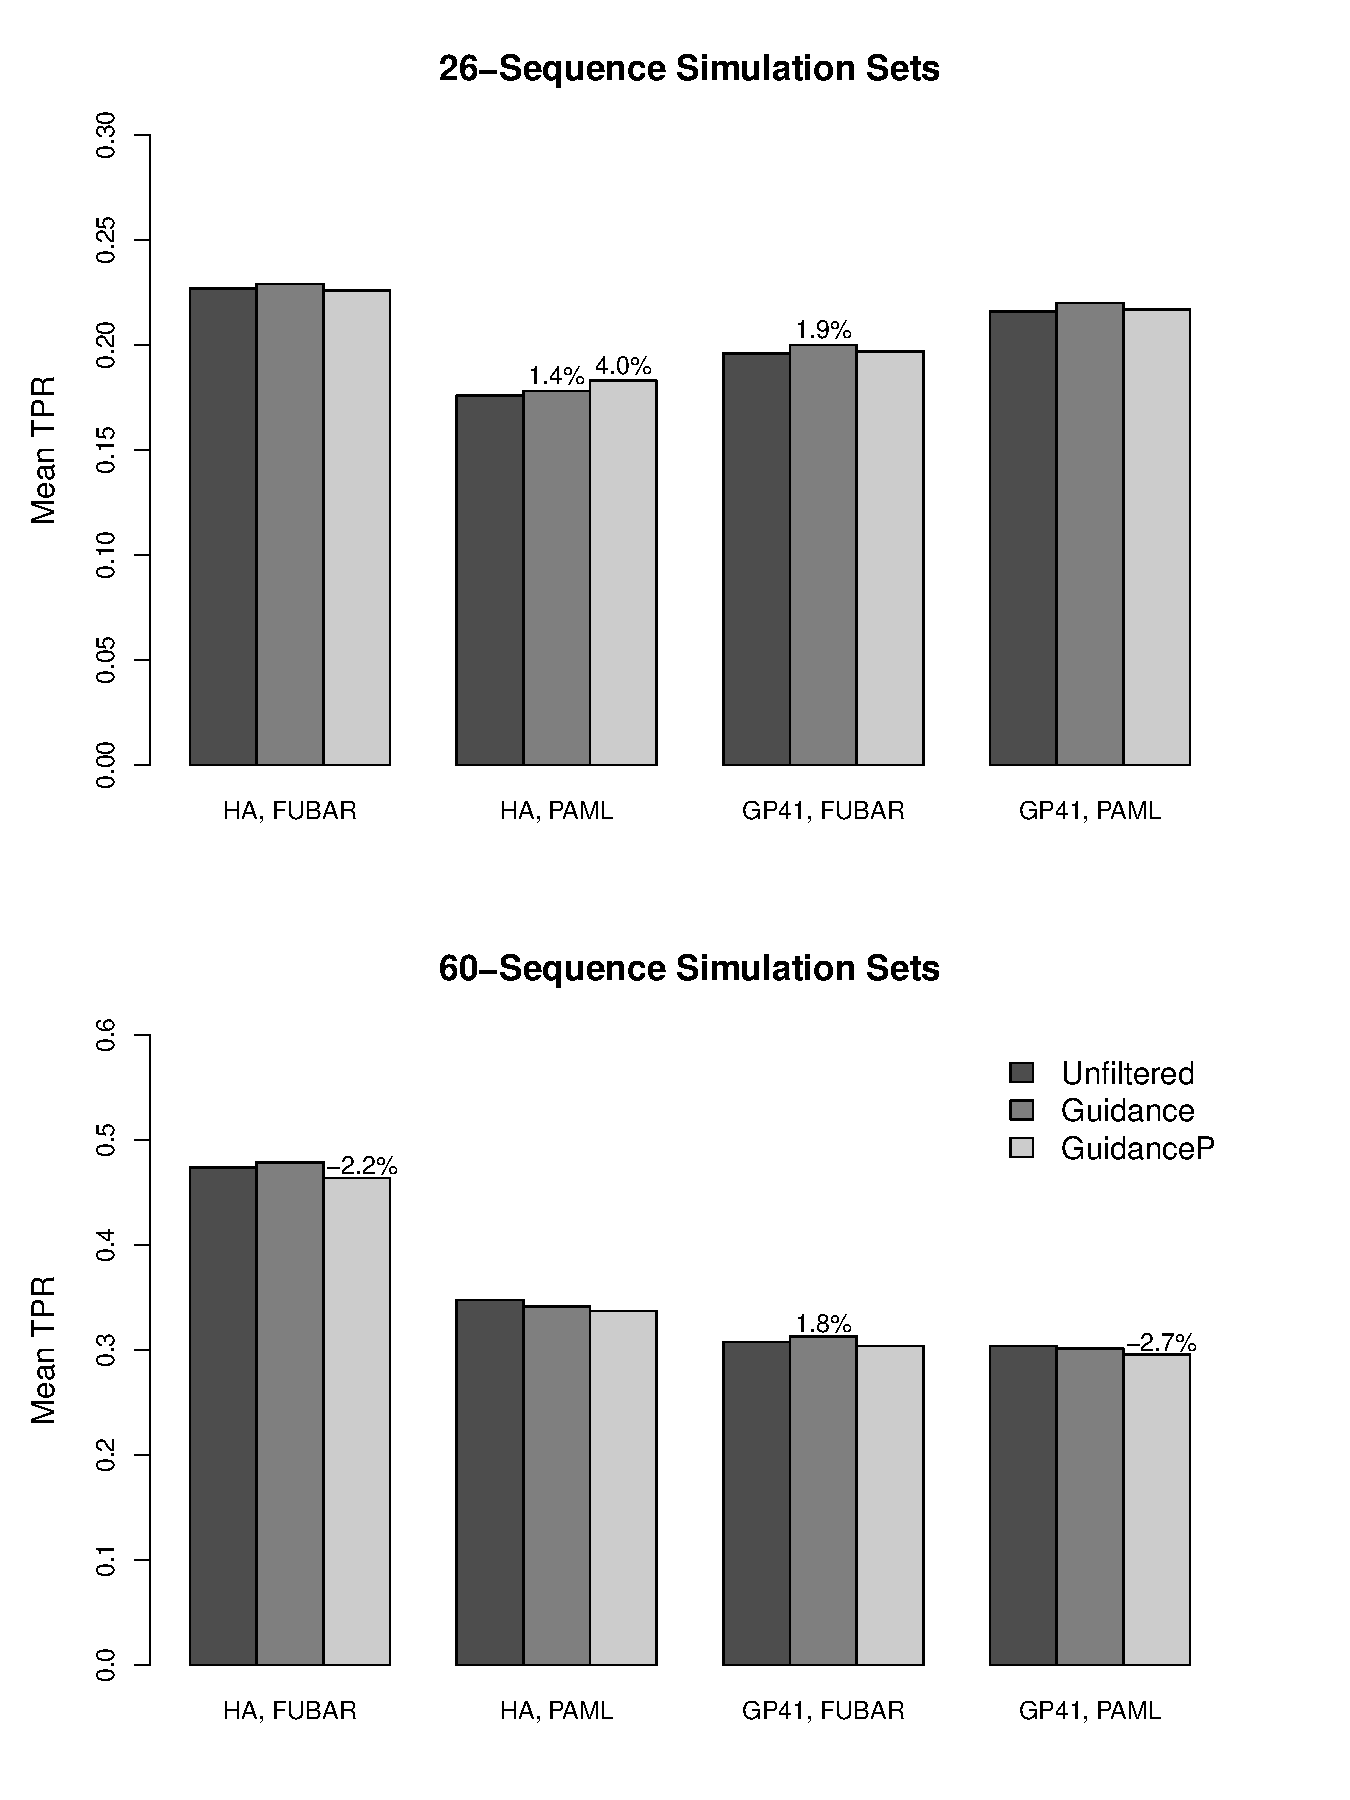
\includegraphics[width=4.75in]{Figures/barplot.pdf}}
\caption{\label{barplot} Mean TPR for and 26- and  60-sequence simulation sets. Percentages, which represent the average percent TPR change from the unfiltered MSAs, are shown only for those changes which are significant. Significance levels are the same as those given in Table \ref{tab:summarystats}. Dark gray bars represent unfiltered MSAs, medium gray bars represents MSAs filtered with Guidance, and light gray bars represent MSAs filtered with GuidanceP.}
\end{figure*}

\bigskip

\begin{figure*}[H]
\centerline{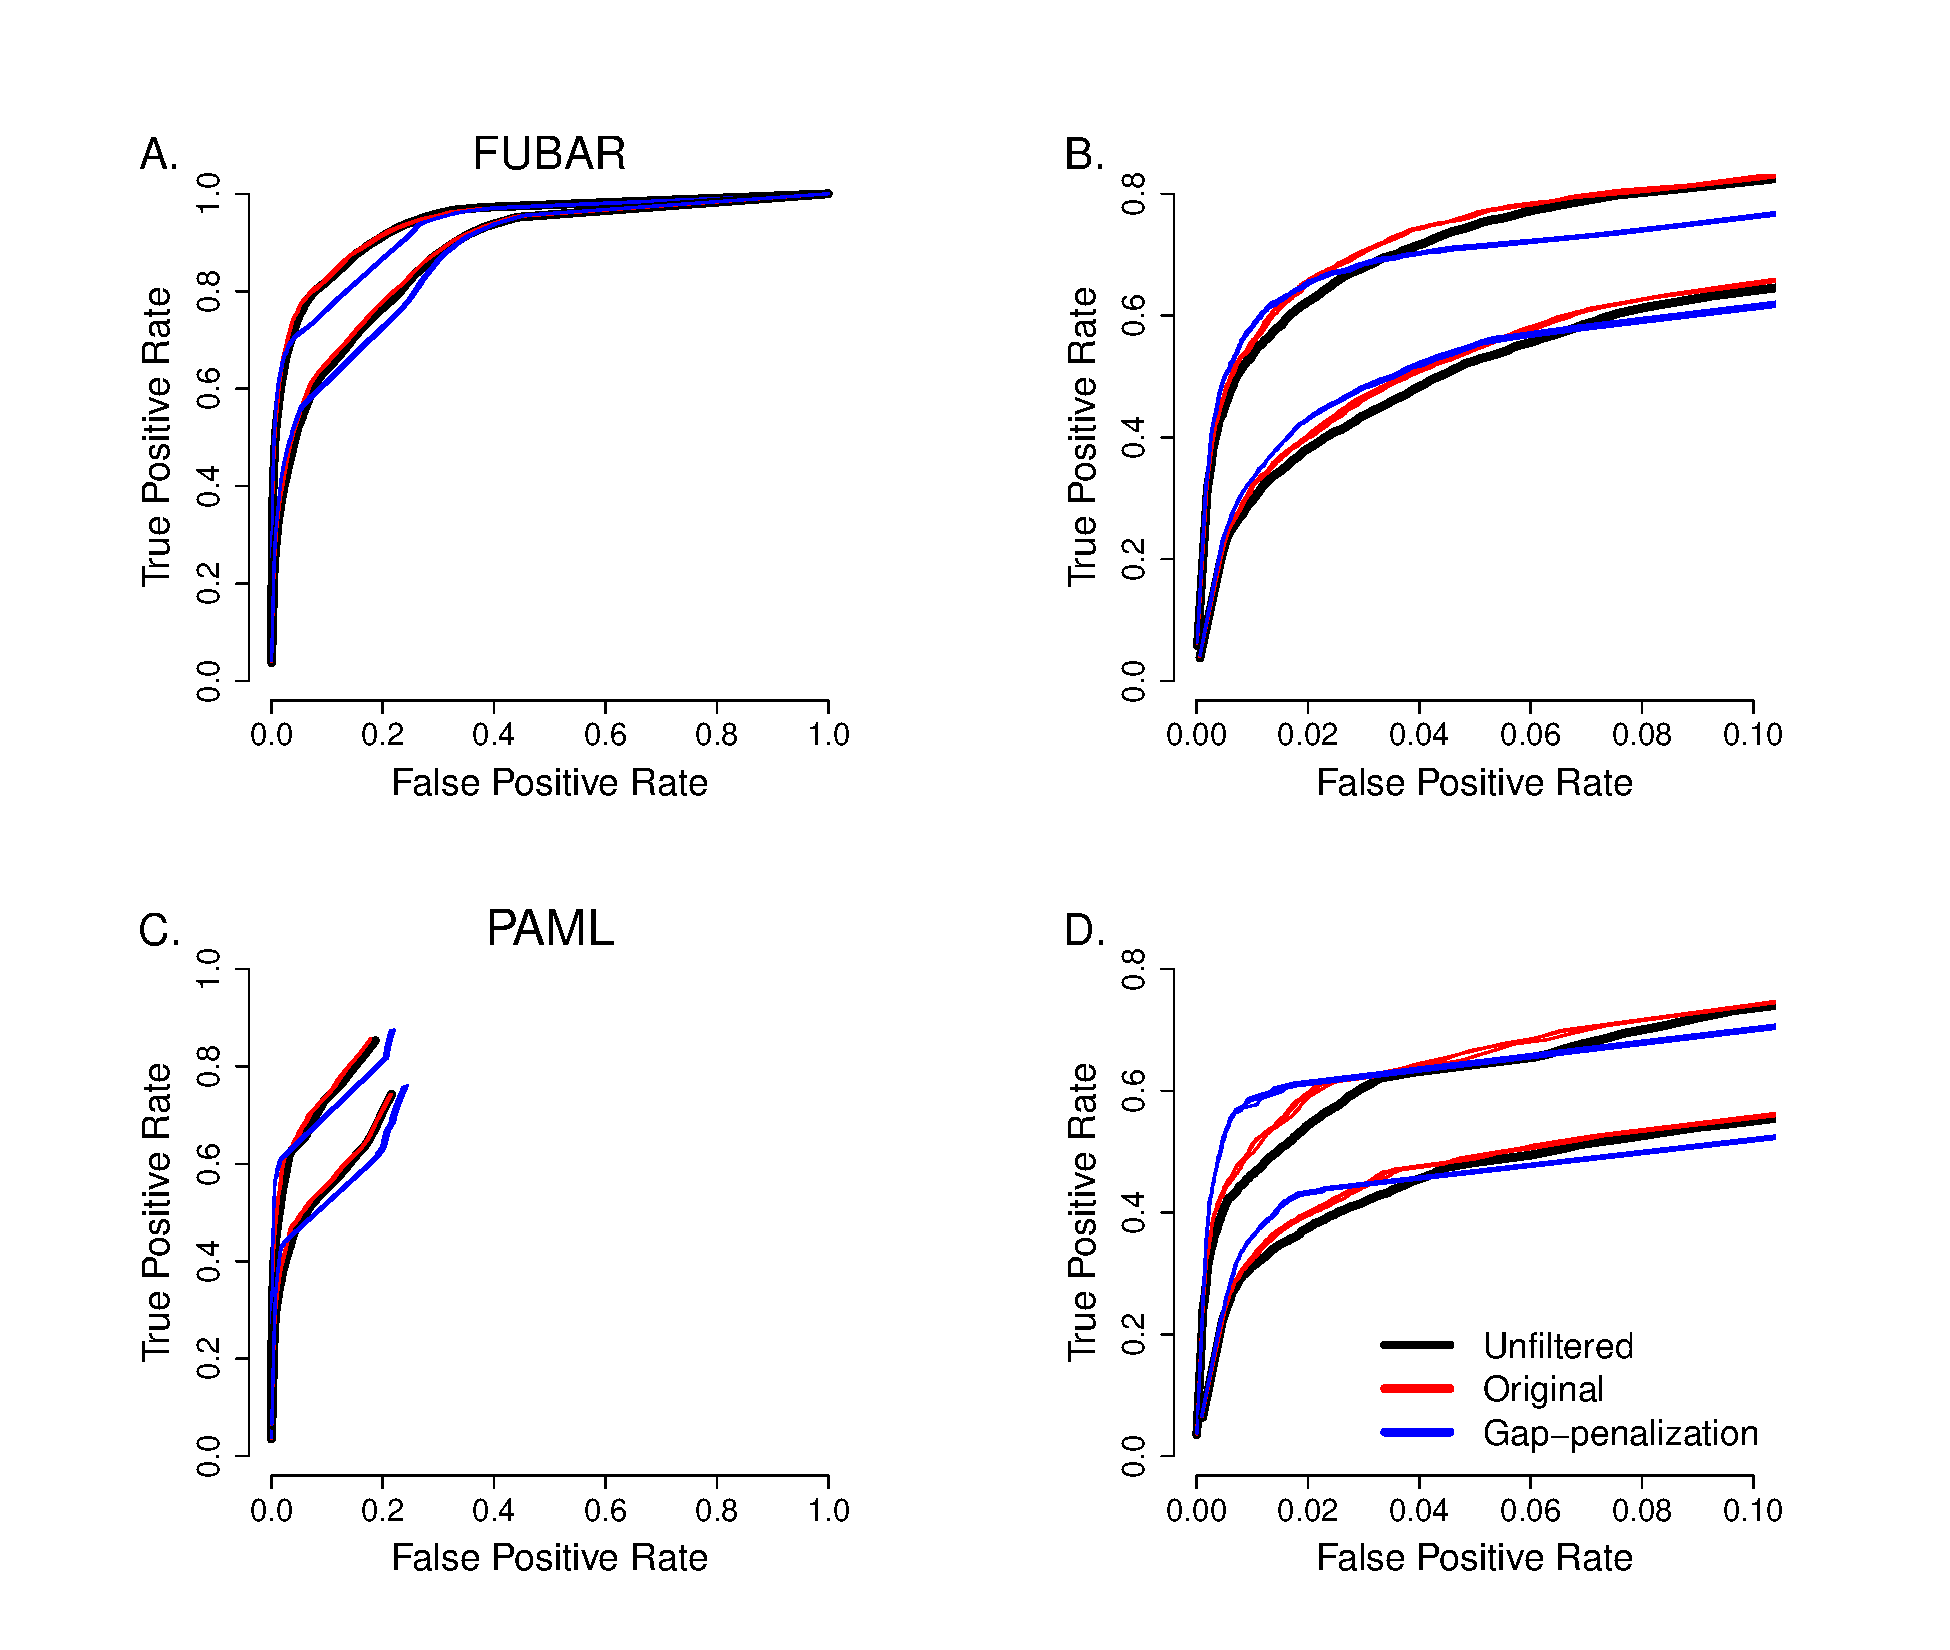
\includegraphics[width=6in]{Figures/ROC_prk.pdf}}
\caption{\label{roc} ROC curves as averaged across the two 60 sequence simulation sets. Within each panels, the top curve represents results from the HA selective profile, and the bottom curve represents results from the GP41 selective profile. Full ROC curves are shown in the left-hand panels. Note that, for the full ROC curves, methods only achieved FPR levels shown. The right-hand panels highlight specifically the low FPR regions ($0--0.1$) of the ROC curves. A-B) ROC curves for positive-selection inf8erence by FUBAR. C-D) ROC curves for positive-selection inference by PAML M8.}
\end{figure*}

\end{document}